\section{TRNG Implementation}

\begin{figure}[t!]
	\centering
	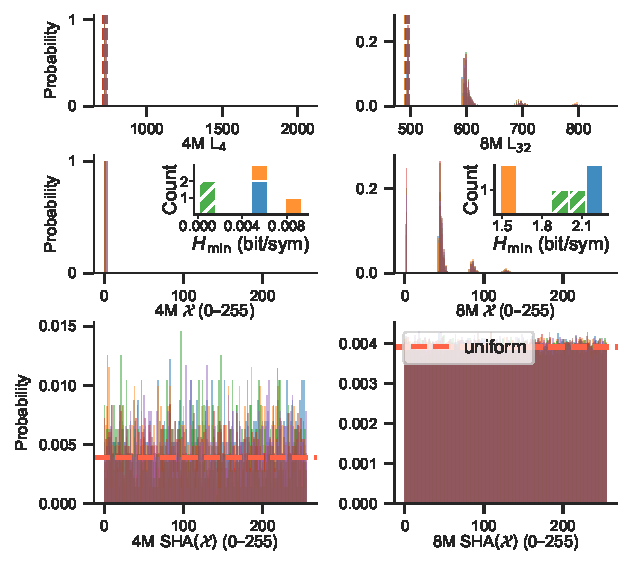
\includegraphics[width=0.9\linewidth]{img/trng_flow_RST_sidebyside.pdf}
	\caption{
		Raw samples (top), symbol mappings and per-region Hmin (middle), and conditioned output (bottom) for 4 fresh 4M (left) and 4 fresh 8M (right) 256B test regions. The $H_{min}$ of each region is colored according the chip in which the region is locate. Two regions are measured at 50\textdegree~C are colored green with a striped texture. NIST 90b reports extremely low $H_{min}$ for all tested regions in the 4M modules, making the required data collection for the NIST-22 and PractRand impractical, while the 8M performs extremely well.
		\label{fig:eval-entropy}
	}
\end{figure}

\subsection{Entropy Source}
We now define our entropy source concretely. For all 4M (8M) modules, we
identify 4-word (32-word) bursts of weight-$D_{min}$ (weight-$D_{min}$)
codewords as the highest entropy rate operation. The entropy source is
derived from a fixed, 256-byte-aligned, contiguous region in the memory.
The region is driven with a fixed repeating sequence and latency
measurements are captured for every bursted write. The sequence
$S_{opt}$ is selected from the characterization performed in
Section~\ref{sec:opt-burst} and is driven as it was in
Algorithm~\ref{alg:burst}, although all other burst configurations are
removed. However, rather than applying a full 256-byte write transaction
for all writes and rotating by a fixed word-width chunk (as in Section
\ref{sec:opt-burst}) we now stride the 256-byte region by exactly the
burst width in a non-overlapping manner. As there is no longer a fixed
1-word rotation this efficient runtime sequence incurs only $r_t$ (see
Eqn. \ref{eqn:rt}) cycles on each bitcell. This significantly reduces
the size of the runtime write pattern sequence as single-word rotation
requires wrapping capabilities that are only possible if a full 256-byte
burst operation is performed.

As the sequence is wear-leveled within and between words, repeating
complete sequences guarantees that each TRNG access is wear-leveled. We
evaluate three 4M and three 8M modules as TRNG sources using this
runtime sequence. One module of each density is placed in a temperature
chamber and heated to $55$\textdegree C. For each module we randomly
select two fresh (unworn) 256-byte regions. Each region on each module
is evaluated as a unique entropy source.

\subsection{Burn-in \& Symbol Characterization}
The results in Figures \ref{fig:opt-burst4m} and \ref{fig:opt-burst8m}
demonstrated that a significant gap in entropy efficiency is closed by
burning in the ReRAM module with 50k full turnover sequences over the
entropy source region. If we were to profile before closing that gap, we
would significantly underestimate the $H_{min}$ of the source.
Therefore, we mandate a 50k full turn-over burn-in phase for each
entropy source before it may be used.

\subsection{Characterization \& Symbol Mapping}
After burn-in, each entropy source undergoes a characterization pass in
which $S_{opt}$ is applied 10 times to establish observed minimum and
maximum write latencies. Latencies are then mapped to 1-byte symbols via
a bin assignment scheme. The lowest bin is reserved for underflow
monitoring. The remaining 255 bins are distributed across the observed
latency range with a minimum bin-width equal to the measurement
resolution of the module. If the observed range is narrower than 255
bins at this resolution, surplus bins are allocated to capture future
rare high-latency switching events. If the observed range exceeds 255
bins at minimum resolution, the bin-width is increased to the smallest
integer multiple of the measurement resolution that accommodates all
observed latencies. Because this scheme merges adjacent latency values
into shared bins and saturates extreme measurements into the reserved
boundary bins, it yields conservative entropy estimates.

\subsection{Conditioning}
Following SP 800-90B~\cite{nist90b}, raw latency samples are conditioned
using SHA-256 as a vetted conditioning component. Per the standard's
vetted conditioning requirements,
\begin{equation}
	\left\lceil\frac{256 + 64}{H_{min}}\right\rceil
\end{equation}
1-byte symbols are submitted to the hash function per 256-bit output block, where 256 is the output length of SHA-256 and the additional 64-bit margin ensures that the conditioning output is full-entropy with adversarial advantage bounded by $2^{-64}$. Each symbol is derived from a single write latency measurement, concatenated with preceding symbols, and hashed to produce the final output bitstring. This conditioning step removes residual bias and correlation in the raw timing observations, yielding uniformly distributed output suitable for use as TRNG entropy source.

\subsection {Measurement Collection}
We collect all latency measurements across the two randomly selected
regions of the 6 ReRAM modules under test. Figure \ref{fig:eval-entropy}
demonstrates the latency, symbol, and output distributions of the TRNG
for the 4M and 8M modules. Additionally, the $H_{min}$ reported by
NIST-90b for each device is The 4M exhibits near-zero latency variance
under the isolated runtime sequence, in contrast to the entropy
efficiency observed during characterization. The 8M, by contrast,
produces latency distributions under runtime conditions that closely
match its characterization-phase behavior, validating the evaluation
methodology and confirming that the 4M divergence is a module-specific
effect rather than a measurement artifact. We attribute the 4M result to
stimulus-conditioned stochasticity: the characterization regime
exercises the full range of burst configurations, whereas the fixed
repeating $S_{opt}$ sequence does not. This sensitivity to stimulus
disqualifies the 4M as a viable TRNG platform and motivates the 8M as
the preferred implementation target. While entropy does exist, the
methods here are likely less effective than those explored in
\cite{tolga2024trng}, where aggressive debiasing was implemented. The
contrast between the two modules further validates the importance of
runtime evaluation: characterization-phase estimates alone would have
significantly overstated the 4M's operational entropy rate.